\documentclass{article}
\usepackage[utf8]{inputenc}
\usepackage[english]{babel}
\usepackage{amsmath,amsfonts,amssymb,amsthm}
\usepackage{mathtools}
\usepackage{fancyhdr}
\usepackage{commath}
\usepackage[sc,osf]{mathpazo}
\usepackage{graphicx}
\usepackage{rotating}
\usepackage{float}
\usepackage{subcaption}
\restylefloat{table}
\usepackage{multicol}
\usepackage[dvipsnames]{xcolor}
\usepackage[colorinlistoftodos]{todonotes}
\usepackage{vmargin}  % Administrar márgenes
\setpapersize{A4} % Definir tamaño del papel
\setmargins{2.5cm} % Margen izquierdo
{1cm} % Margen superior
{16.5cm} % Área de impresión horizontal
{23.42cm} % Area de impresión vertical
{15mm} % Encabezado
{5mm} % Espacio entre el encabezado y el texto
{10pt} % Pie de página
{3mm} % Espacio entre el pie de página y el texto

\pagestyle{fancy}
\fancyhf{}
\rhead{

\includegraphics[width=4cm,height=1cm]{cropped-iitpal-at-prutor-logo.png}
}
\lhead{Circles | Class XI}
\rfoot{}
\begin{document}
\section{Terminology}
\begin{figure}[H]
    \centering
    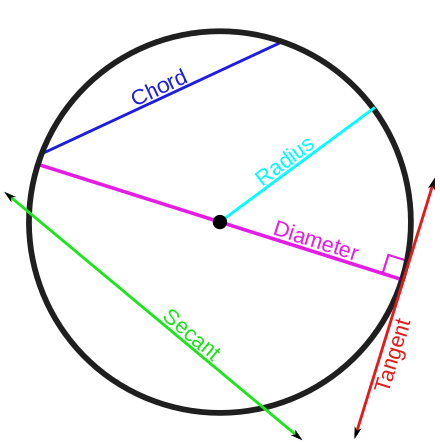
\includegraphics[scale=0.5]{CIRCLE_LINES.png}
    \caption{Circle Terminology}
\end{figure}
\begin{itemize}
    \item Radius: a line segment joining the centre of a circle with any single point on the circle itself; or the length of such a segment, which is half (the length of) a diameter.
    \item Chord: a line segment whose endpoints lie on the circle, thus dividing a circle into two segments.
    \item Diameter: a line segment whose endpoints lie on the circle and that passes through the centre; or the length of such a line segment. This is the largest distance between any two points on the circle. It is a special case of a chord, namely the longest chord for a given circle, and its length is twice the length of a radius.
    \item Sector: a region bounded by two radii of equal length with a common center and either of the two possible arcs, determined by this center and the endpoints of the radii.
    \item Tangent: a co-planar straight line that has one single point in common with a circle ("touches the circle at this point").
\end{itemize}
\section{Circle Equation}

\subsection{Center Radius Form}
\begin{equation*}
    (x-a)^2+(y-b)^2=r^2
\end{equation*}
\subsection{Parametric Form}
\begin{align*}
    x=a+r cos\theta\\
    y=b+r sin\theta
\end{align*}
Here $\theta$ is the parametric variable that ranges from $0$ to $2\pi$.
\subsection{General Form}
\begin{equation*}
    x^2 + y^2+2gx+2fy+c=0
\end{equation*}
By comparing with center-radius form we can see that, center of the circle is (-g,-f) and radius $\sqrt{g^2+f^2-c}$.
\end{document}